\documentclass[bigger]{beamer}
%\documentclass[handout]{beamer}
\setbeamertemplate{bibliography item}{}
\usepackage[utf8]{inputenc}
\usepackage[english]{babel}
\usepackage{multirow}
\usepackage{synttree}
\usepackage{booktabs}
\usepackage[backend=bibtex,natbib,style=authoryear]{biblatex}
\usetheme{Warsaw}
%\usefonttheme[onlylarge]{structuresmallcapsserif}
\newcommand{\wigegraph}[1]{\begin{figure}[h]
\centering\includegraphics[width=\textwidth]{#1}\end{figure}}
% Ez most valamiert besz.rt, ugyhogy kikommentalom:
%\AtBeginSection[]{\frame{\frametitle{Outline}\tableofcontents[current]}}

\AtBeginPart{\frame{\partpage}} 

\usepackage{tikz}
\usepackage{tikz-qtree}
\usepackage{xspace}

\bibliography{ml}

\newcommand{\defl}{\texttt{dep\_to\_4lang}\xspace}
\newcommand{\difl}{\texttt{dict\_to\_4lang}\xspace}
\newcommand{\tfl}{\texttt{text\_to\_4lang}\xspace}
\newcommand{\tefl}{\texttt{text\_to\_4lang}\xspace}
\newcommand{\fl}{\texttt{4lang}\xspace}

\newcommand{\edge}[3]{\texttt{#1}~$\xrightarrow#2$~\texttt{#3}}
\newcommand{\twoedges}[4]{\texttt{#1}~$\overset{#2}{\underset{#3}{\rightleftharpoons}}$~\texttt{#4}}
\newcommand{\bin}[3]{
    \texttt{#2}~$\xleftarrow1$~\texttt{#1}~$\xrightarrow2$~\texttt{#3}}

\newcommand{\todo}[1]{\textbf{TODO: #1}}

%\usepackage{apacite}
%\let\cite\shortcite  % to get "et al." for more than two authors
%\let\citeA\shortciteA
\begin{document}

\title{Machine Comprehension using semantic graphs}
\author{\'Ad\'am Kov\'acs \\ Kinga G\'emes \\ G\'abor Recski}
\institute{\texttt{kovacs.adam@aut.bme.hu}, \texttt{kinga.andrea.gemes@gmail.com}, \texttt{recski@aut.bme.hu}}

\date{AACS19\\21.06.2019.}

%-----------------------

\begin{frame} 

\titlepage 

\end{frame} 
%----------------------

%-----------------------

\begin{frame} 

    \frametitle{Our contribution} 
    \begin{itemize}
        \pause \item Defining graph based semantic models
        \pause \item Evaluation of our models on a machine comprehension task
        \pause \item Integrating our model to a state-of-the-art system
        \pause \item Results show some improvement on the task
    \end{itemize}

\end{frame} 

%-----------------------
\begin{frame}
	\frametitle{The machine comprehension task \citep{Chen:2018, Wang:2018}}
	\textbf{Text:} "Today we decided to paint the extra room in our house. Were going to have visitor coming next month so hopefully the painting ain't that smelly anymore. I made sure that the wall is clean and clear of all the nuisance. We already bought the pain and we decided the new wall pain is sky blue. My husband is putting newspaper on the floor to avoid any spill on our floor/carpet....." \\
	\textbf{Question:} "Did anyone help him?" \\
	\textbf{1st answer:} "It was the narrator and her husband" \\
	\textbf{2nd answer:} "No, he worked alone."
\end{frame}

%---------------------

\begin{frame}
	\frametitle{The machine comprehension task \citep{Chen:2018, Wang:2018}}
	\begin{columns}
		\begin{column}{0.6\textwidth}
			\begin{itemize}
				\pause \item \textbf{2018-as Semeval Task}
				\begin{itemize}
					\item \textit{Machine comprehension using commonsense knowledge}
				\end{itemize}
				\pause \item Simple multi-choice questions based on short stories
			\end{itemize}
		\end{column}
		\begin{column}{0.5\textwidth}
			\begin{itemize}
				\pause \item The best two systems
				\begin{itemize}
					\item \texttt{HFL-RC}
					\item \texttt{Yuanfudao}
				\end{itemize}
				\pause \item \textbf{MCScript}
				\begin{itemize}
					\item training and test data
				\end{itemize}
			\end{itemize}
		\end{column}
	\end{columns}
	
\end{frame}

%-----------------------
{
\setbeamerfont{frametitle}{size=\small}

\begin{frame}
    \frametitle{\fl: the formalism \citep{Kornai:2010,Kornai:2015a}}
\pause Directed concept graphs with 3 types of edges 
\begin{itemize}
    \pause \item type 0 edge
        \begin{itemize}
            \pause \item property: \texttt{dog}~$\xrightarrow0$~\texttt{large}
            \pause \item \texttt{IS\_A} relation (hypernym): \texttt{dog}~$\xrightarrow0$~\texttt{mammal}
            \pause \item predicate: \texttt{dog}~$\xrightarrow0$~\texttt{bark}
        \end{itemize}
    \pause \item type 1 and type 2 edges connect binary predicates with their arguments.
\end{itemize}
\pause \begin{figure}
\centering
    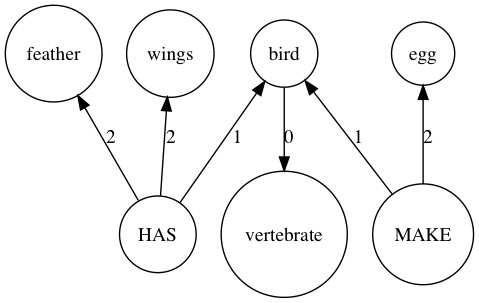
\includegraphics[scale=0.385]{pics/bird.jpg}
\end{figure}
\end{frame}
}
%-----------------------
\begin{frame}
\frametitle{The \fl service}
		\begin{itemize}
			\pause \item Service built on the \tefl module
			\pause \item Highly automated graph generation
			\pause \item Online demo
			\begin{itemize}
				 \item \url{http://4lang.hlt.bme.hu}
			\end{itemize}
			\pause \item Github
			\begin{itemize}
				\item \url{https://github.com/adaamko/4lang}
			\end{itemize}
		\end{itemize}

\end{frame}
%-----------------------
%-----------------------
\begin{frame}
\frametitle{The \fl service}
\begin{columns}
	\begin{column}{0.3\textwidth}
		\pause My poor wife!
		\pause 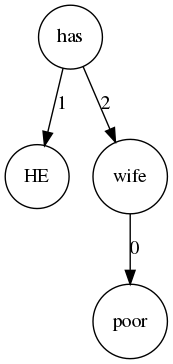
\includegraphics[scale=0.4]{pics/wifepoor.png}
	\end{column}
	\begin{column}{0.4\textwidth}
		I feel bad for my wife!
		\pause 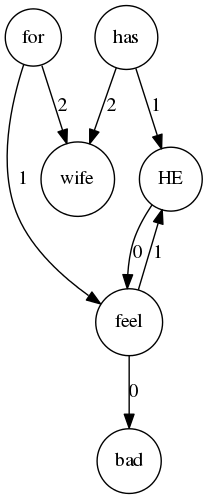
\includegraphics[scale=0.4]{pics/feelbad.png}
	\end{column}
\end{columns}

\end{frame}
%-----------------------
\begin{frame}
\frametitle{Defined metrics}
\begin{columns}
	\begin{column}{0.5\textwidth}
		\begin{itemize}
			\pause \item \textbf{Goal}
			\begin{itemize}
				\item is the statement a consequence of the hypothesis?
			\end{itemize}
			\pause \item \textbf{Implementation}
			\begin{itemize}
				\item Graph similarity
				\item What makes two graphs similar?
			\end{itemize}
		\end{itemize}
	\end{column}
	\begin{column}{0.5\textwidth}
		\begin{itemize}
			\pause \item My poor wife! (G1)
			\pause \item I feel bad for my wife! (G2)
			\pause \item \[\frac{|E(G_1)\cap E(G_2)|}{|E(G_2)|}\]			
		\end{itemize}
	\end{column}
\end{columns}

\end{frame}
%-----------------------
\begin{frame}
\frametitle{Expanded graphs, the "expand" function}
\begin{columns}
	\begin{column}{0.1\textwidth}
		\pause 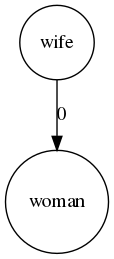
\includegraphics[scale=0.4]{pics/wife.png}
	\end{column}
	\begin{column}{0.1\textwidth}
	\pause \[\Rightarrow\]
	\end{column}
	\begin{column}{0.2\textwidth}
		\pause 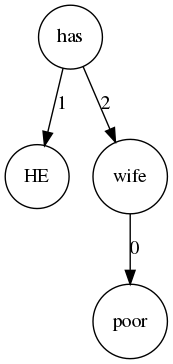
\includegraphics[scale=0.4]{pics/wifepoor.png}
	\end{column}
	\begin{column}{0.1\textwidth}
		\pause \[\Rightarrow\]
	\end{column}
	\begin{column}{0.3\textwidth}
	\pause 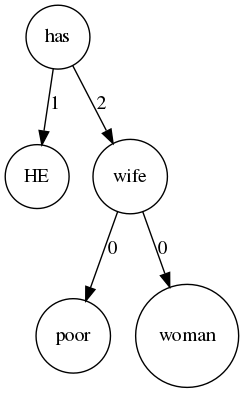
\includegraphics[scale=0.4]{pics/wifeexp.png}
	\end{column}
\end{columns}
\end{frame}

%--------------------------------------------

\begin{frame}
    \frametitle{Baseline}
    \begin{figure}
        \centering
        \small
            \begin{itemize}
				\item Merged graph for all question-answer pair
				\item The "more" similar is the correct answer
				\item \textbf{68,3} accuracy score
			\end{itemize}
            \begin{columns}
				\begin{column}{0.2\textwidth}
					\pause 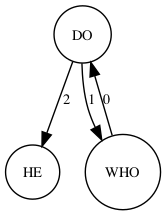
\includegraphics[scale=0.5]{pics/didit.png}
				\end{column}
				\begin{column}{0.2\textwidth}
				\pause \[\Rightarrow\]
				\end{column}
				\begin{column}{0.2\textwidth}
					\pause 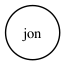
\includegraphics[scale=0.5]{pics/jon.png}
				\end{column}
				\begin{column}{0.2\textwidth}
					\pause \[\Rightarrow\]
				\end{column}
				\begin{column}{0.3\textwidth}
				\pause 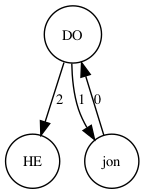
\includegraphics[scale=0.5]{pics/jondid.png}
				\end{column}
			\end{columns}
        \label{fig:method}
        \end{figure}
\end{frame}

%-----------------------

\begin{frame}
	\frametitle{Deep learning}
	\begin{itemize}
		\pause \item Widely used method
		\pause \item State-of-the-art in Natural Language Processing
		\pause \item RNN handles sequential data the best
		\begin{itemize}
			\pause \item LSTM
			\pause \item Attention
		\end{itemize}
	\end{itemize}
\end{frame}

%-----------------------

\begin{frame}
	\frametitle{Yuanfudao system}
	\begin{figure}[h!]
		\centering
		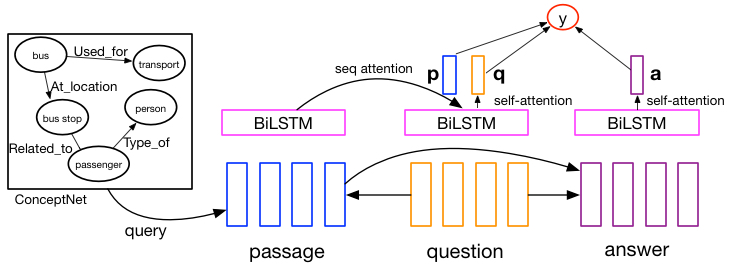
\includegraphics[scale=0.4]{pics/TriAN.jpg}
		\caption{The structure of the system}
		\label{fig:dnn}
	\end{figure}
\end{frame}
%-----------------------
\begin{frame}
	\frametitle{Modifications}
	\begin{itemize}
		\pause \item \fl similarity score calculated between words during the pre-processing
		\pause \item New embedding layer for the \fl similarities
		\pause \item Expansion of the RNN layer, that the corresponding RNN gets the \fl embedding's output
	\end{itemize}
\end{frame}


%-----------------------

\begin{frame}
	\frametitle{Results}
	\begin{table}[!h]
		\centering
		\begin{tabular}{ | l | c | c | }
			\hline
			model & dev & test \\ \hline \hline
			TriAN, no ConceptNet & 82.8\% & 80.2\% \\ \hline
			TriAN, with ConceptNet & 82.7\% & 80.5\% \\ \hline
			\textbf{TriAN, with 4lang} & \textbf{83.2\%} & \textbf{80.9\%} \\ \hline
			TriAN, with both & 83.1\% & 80.8\% \\ \hline
		\end{tabular}
		\caption{Effect of \texttt{4lang} and \texttt{ConceptNet} on results}
		\label{tabl:res}
	\end{table}
\end{frame}

\begin{frame}
	\frametitle{Results}
	\begin{table}[!h]
		\centering
		\begin{tabular}{| l | c | c |}
			\hline
			model & dev & test \\ \hline \hline
			TriAN, no ConceptNet & 83.7\% & 81.9\% \\ \hline
			TriAN, with ConceptNet & 82.5\% & 80.3\% \\ \hline
			TriAN, with 4lang & 84.2\% & 81.5\% \\ \hline
			\textbf{TriAN, with both} & \textbf{83.4\%} & \textbf{82.9\%} \\ \hline
		\end{tabular}
		\caption{Effect of \texttt{4lang} and \texttt{ConceptNet} on the pretrained models}
		\label{tabl:pretrained}
	\end{table}
\end{frame}

\begin{frame}
	\frametitle{Results}
	\begin{table}[!h]
		\centering
		\begin{tabular}{ | l | c | }
			\hline
			pretrained, ensembled model & test \\ \hline \hline
			TriAN, no ConceptNet & 82.95\% \\ \hline
			TriAN, with ConceptNet &  83.697\% \\ \hline
			TriAN, with 4lang & 82.8\% \\ \hline
			\textbf{TriAN, with both} & \textbf{83.73\%} \\ \hline
		\end{tabular}
		\caption{The effect of \texttt{4lang} and \texttt{ConceptNet} on the pretrained and ensembled models}
		\label{tabl:pretrained_ensembled}
	\end{table}
\end{frame}

%-----------------------
\begin{frame}
\frametitle{Summary}
	\begin{itemize}
	    \pause \item Automated method and metric for measuring similarity.
	    \pause \item Strong baseline on the machine comprehension task
	    \pause \item Using out baseline method in the state-of-the-art system, seeing some improvement
	    \pause \item A code is available at \url{https://github.com/adaamko/4lang} \\ \url{https://github.com/GKingA/commonsense-rc}
	    \pause \item Live Rest API and online demo \url{http://4lang.hlt.bme.hu}
	\end{itemize}

\end{frame}
%-----------------------
%-----------------------
\begin{frame}
    \frametitle{Thank you for your attention!}
    \AtNextBibliography{\tiny}
    \printbibliography
\end{frame}
%-----------------------


\end{document}






